\chapter{Deseño}
Neste capítulo explícase a arquitectura da plataforma comezando por unha visión xeral da mesma para despois comentar máis en detalle o modelo de datos, o deseño do servidor e a aplicación Android.


\section{Arquitectura xeral}

A nosa plataforma consta dos seguintes elementos conectados entre si:
\begin{itemize}
	\item Servidor de base de datos (POIs e percorridos).
	\item Aplicación Android para visualización e edición de datos.
	\item Sistema de autenticación (GoogleAuth).
	\item Sistema de localización en interiores (Situm).
\end{itemize}

A aplicación Android precisa o servidor para a recuperación dos datos propios da plataforma e o sistema de localización en interiores para poder funcionar. O sistema de autenticación de Google está relacionado coa aplicación Android, onde comeza ese proceso, e co servidor, que realiza o último paso. Pódense observar estas conexións entre os elementos na figura~\ref{fig:arq_xeral}):


\begin{figure}[tb] 
	\begin{center}
		\includegraphics[width=0.65\textwidth]{figures/arqXeral}
		\caption{Arquitectura xeral da plataforma Caronte para a guía de museos.}
		\label{fig:arq_xeral}
	\end{center}
\end{figure}

O servidor encárgase de recuperar e procesar a información que precisa a aplicación para o seu funcionamento. Esta información é almacenada nunha base de datos PostgreSQL. Aparte de recuperar esta información, tamén se encarga de inserir os datos indicados polo usuario dentro da aplicación. Para permitir a comunicación coa aplicación Android e que o usuario poida recibir e modificar esa información, publícanse uns servizos web a través dunha API REST.

A aplicación Android é o punto de interacción do usuario coa nosa plataforma. Presenta a información recuperada do servidor ao usuario e permite a súa modificación, enviando de novo os datos para a súa persistencia. Tamén é a encargada de tratar cos servizos de Situm que permiten a localización e o guiado en interiores, recuperando a información necesaria e presentándolla ao usuario.

O sistema de autenticacion de Google permite a recuperación de información propia do usuario a través dunha conta de Google. Ao utilizar este sistema, pódese dispoñer da información dunha conta de usuario e gardala no noso servidor, polo que se pode utilizar para asociar permisos ou gardar outra información relacionada.


\section{Modelo de datos}
Neste punto exporase o modelo de datos da plataforma que se seguiu á hora da creación da base de datos. Na figura ~\ref{fig:modelo_datos} pódese observar o diagrama entidade relación. Dividirase a explicación

\begin{figure}[tb] 
	\begin{center}
		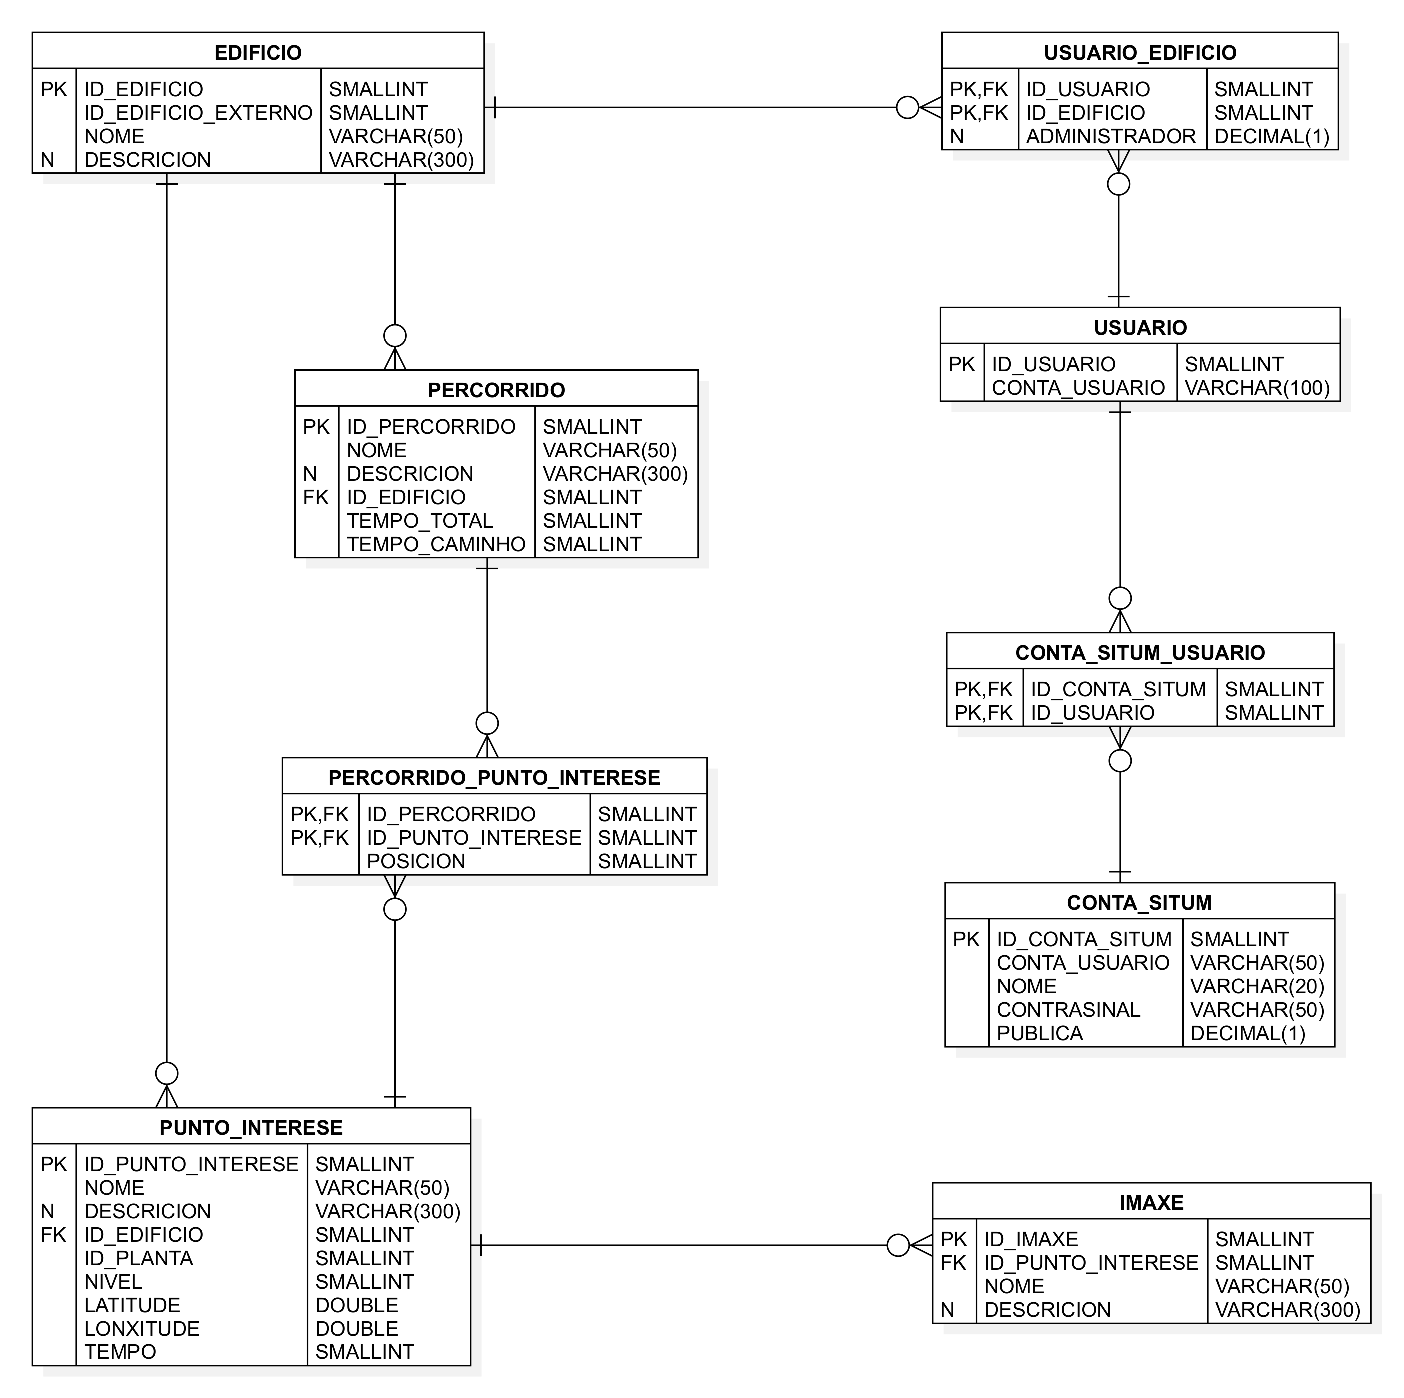
\includegraphics[width=0.95\textwidth]{figures/BD/diagramaEntidadeRelacion}
		\caption{Modelo de datos da plataforma Caronte.}
		\label{fig:modelo_datos}
	\end{center}
\end{figure}

\subsection{EDIFICIO}
Nesta entidade gardarase a información básica dos edificios que se tratan na aplicación. Aparte dos datos propios creados para a plataforma tamén se garda o identificador do edificio dentro do sistema Situm, que permite relacionar os edificios de Caronte cos de Situm.

As columnas das que se compón este entidade son:
\begin{itemize}
	\item ID\_EDIFICIO: Chave primaria autoxerada da táboa. De tipo SMALLINT (short). É o identificador do edificio dentro do sistema de Caronte. Non pode ter valor nulo.
	\item ID\_EDIFICIO\_EXTERNO: De tipo SMALLINT (short). É o identificador do edificio dentro do sistema de Situm.
	\item NOME: De tipo VARCHAR (string) con límite de 50 caracteres. É o texto que se visualizará na aplicación e que permite ao usuario a distinción entre edificios. Non pode ter valor nulo.
	\item DESCRICION: De tipo VARCHAR (string) con límite de 300 caracteres. Un breve texto explicativo sobre o edificio. Pode ter valor nulo.
\end{itemize}

\subsection{USUARIO}
Nesta entidade gardarase a conta de usuario de Google coa que alguén se autentica na aplicación. Só se gardará o nome desa conta.

As columnas das que se compón este entidade son:
\begin{itemize}
	\item ID\_USUARIO: Chave primaria autoxerada da táboa. De tipo SMALLINT (short). É o identificador do usuario dentro do sistema de Caronte. Non pode ter valor nulo.
	\item CONTA\_USUARIO: De tipo VARCHAR (string) con límite de 100 caracteres. Correspóndese coa conta de correo de Google do usuario que se autentica na aplicación. Non pode ter valor nulo.
\end{itemize}

\subsection{USUARIO\_EDIFICIO}
Nesta entidade gardarase información sobre as accións que pode levar a cabo un usuario sobre un edificio concreto. A información desta entidade é a que indica se un usuario é un xestor de contido sobre un edificio.

As columnas das que se compón este entidade son:
\begin{itemize}
	\item ID\_USUARIO: Forma parte da chave primaria da entidade. Chave foránea da táboa USUARIO. De tipo SMALLINT (short). Non pode ter valor nulo.
	\item ID\_EDIFICIO: Forma parte da chave primaria da entidade. Chave foránea da táboa EDIFICIO. De tipo SMALLINT (short). Non pode ter valor nulo.
	\item ADMINISTRADOR: De tipo DECIMAL con límite 1 (boolean). Indica se o usuario é xestor de contido sobre o edificio.
\end{itemize}


\subsection{PUNTO\_INTERESE}
Nesta entidade gardarase información sobre os puntos de interese creados sobre un edificio e a súa localización exacta no planeta. Un punto de interese só pode pertencer a un único edificio e estará localizado nunha das súas plantas.

As columnas das que se compón este entidade son:
\begin{itemize}
	\item ID\_PUNTO\_INTERESE: Chave primaria autoxerada da táboa. De tipo SMALLINT (short). É o identificador do punto de interese. Non pode ter valor nulo.
	\item NOME: De tipo VARCHAR (string) con límite de 50 caracteres. É o texto que se visualizará na aplicación e que permite ao usuario a distinción entre puntos de interese. Non pode ter valor nulo.
	\item DESCRICION: De tipo VARCHAR (string) con límite de 300 caracteres. Un breve texto explicativo sobre o punto de interese. Pode ter valor nulo.
	\item ID\_EDIFICIO: Chave foránea da táboa EDIFICIO. De tipo SMALLINT (short). Permite identificar o edificio no que se atopa o punto. Non pode ter valor nulo.
	\item ID\_PLANTA: De tipo SMALLINT (short). É o identificador da planta dentro do sistema de Situm. Este dato permite maior rapidez á hora de identificador os puntos dunha planta. Non pode ter valor nulo.
	\item NIVEL: De tipo SMALLINT (short). Indica o número de planta no que se atopa un punto. Non pode ter valor nulo.
	\item LATITUDE: De tipo DOUBLE. Indica a latitude do punto, o que permite unha localización exacta nun mapa. Non pode ter valor nulo.
	\item LONXITUDE: De tipo DOUBLE. Indica a lonxitude do punto, o que permite unha localización exacta nun mapa. Non pode ter valor nulo.
	\item TEMPO: De tipo SMALLINT (short). Indica o tempo en minutos de media que lle leva a un visitante admirar unha obra. Non pode ter valor nulo e o seu valor por defecto é 0.
\end{itemize}


\subsection{PERCORRIDO}
Nesta entidade gardarase información sobre os percorridos dispoñíbeis nos edificios. Un percorrido só pode pertencer a un único edificio e non está limitado a unha única planta. Está composto por varios puntos de interese que se almacenan na táboa do seguinte punto.

As columnas das que se compón este entidade son:
\begin{itemize}
	\item ID\_PERCORRIDO: Chave primaria autoxerada da táboa. De tipo SMALLINT (short). É o identificador do percorrido. Non pode ter valor nulo.
	\item NOME: De tipo VARCHAR (string) con límite de 50 caracteres. É o texto que se visualizará na aplicación e que permite ao usuario a distinción entre percorridos. Non pode ter valor nulo.
	\item DESCRICION: De tipo VARCHAR (string) con límite de 300 caracteres. Un breve texto explicativo sobre o percorrido. Pode ter valor nulo.
	\item ID\_EDIFICIO: Chave foránea da táboa EDIFICIO. De tipo SMALLINT (short). Permite identificar o edificio no que se atopa o percorrido. Non pode ter valor nulo.
	\item TEMPO\_TOTAL: De tipo SMALLINT (short). Indica o tempo en minutos de media que lle leva a un visitante realizar todo o percorrido contando co tempo que pase diante das obras. Non pode ter valor nulo e o seu valor por defecto é 0.
	\item TEMPO\_CAMINHO: De tipo SMALLINT (short). Indica o tempo en minutos de media que lle leva a un visitante realizar todo o percorrido sen contar o tempo que pase diante das obras. Non pode ter valor nulo e o seu valor por defecto é 0.
\end{itemize}


\subsection{PERCORRIDO\_PUNTO\_INTERESE}
Nesta entidade gardarase a relación entre os percorridos e os puntos de interese que os compoñen. É obrigatorio indicar a posición de cada un deses puntos xa que os percorridos están ordenados. Un punto de interese só pode aparecer unha única vez nun percorrido, non se permite a súa repetición. Non hai limitación no numero de percorridos aos que pode pertencer un punto de interese.

As columnas das que se compón este entidade son:
\begin{itemize}
	\item ID\_PERCORRIDO: Forma parte da chave primaria da entidade. Chave foránea da táboa PERCORRIDO. De tipo SMALLINT (short). Non pode ter valor nulo.
	\item ID\_PUNTO\_INTERESE: Forma parte da chave primaria da entidade. Chave foránea da táboa PUNTO\_INTERESE. De tipo SMALLINT (short). Non pode ter valor nulo.
	\item POSICION: De tipo SMALLINT (short). Indica a posición ordenada dun punto de interese dentro dun percorrido. Non pode ter valor nulo.
\end{itemize}


\subsection{CONTA\_SITUM}
Nesta entidade almacénanse as distintas contas de usuario dispoñíbeis na aplicación para o acceso á plataforma de Situm. Con elas permítese o tratamento de distintos edificios. As contas poden ser públicas ou privadas, precisando certo permiso o usuario para poder visualizar estas últimas.

As columnas das que se compón este entidade son:
\begin{itemize}
	\item ID\_CONTA\_SITUM: Chave primaria autoxerada da táboa. De tipo SMALLINT (short). É o identificador da conta de Situm. Non pode ter valor nulo.
	\item CONTA\_USUARIO: De tipo VARCHAR (string) con límite de 50 caracteres. É o correo electrónico que utiliza Situm para autenticarse. Non pode ter valor nulo.
	\item NOME: De tipo VARCHAR (string) con límite de 20 caracteres. É o texto que se visualizará na aplicación e que permite ao usuario a distinción entre contas de Situm. Non pode ter valor nulo.
	\item CONTRASINAL: De tipo VARCHAR (string) con límite de 50 caracteres. É o contrasinal que permite a conexión ao sistema de Situm. Non pode ter valor nulo.
	\item PUBLICA: De tipo DECIMAL con límite 1 (boolean). Indica se a conta de Situm pode ser por calquera usuario ou en cambio debe ter permisos sobre ela. Non pode ter valor nulo.
\end{itemize}


\subsection{CONTA\_SITUM\_USUARIO}
Nesta entidade almacénanse as relacións entre os usuarios e as distintas contas de acceso a Situm sobre as que teñen permiso. Non almacena máis que esa relación. Se o usuario ten algunha conta asociada poderá utilizala para acceder ao sistema.

As columnas das que se compón este entidade son:
\begin{itemize}
	\item ID\_CONTA\_SITUM: Forma parte da chave primaria da entidade. Chave foránea da táboa CONTA\_SITUM. De tipo SMALLINT (short). Non pode ter valor nulo.
	\item ID\_USUARIO: Forma parte da chave primaria da entidade. Chave foránea da táboa USUARIO. De tipo SMALLINT (short). Non pode ter valor nulo.
\end{itemize}


\subsection{IMAXE}
Nesta entidade almacénase a información sobre todas as imaxes subidas. Cada rexistro debe facer referencia a un punto de interese concreto.

As columnas das que se compón este entidade son:
\begin{itemize}
	\item ID\_IMAXE: Chave primaria autoxerada da táboa. De tipo SMALLINT (short). É o identificador da imaxe. Non pode ter valor nulo.
	\item ID\_PUNTO\_INTERESE: Chave foránea da táboa PUNTO\_INTERESE. De tipo SMALLINT (short). Permite identificar o punto de interese ao que fai referencia a imaxe. Non pode ter valor nulo.
	\item NOME: De tipo VARCHAR (string) con límite de 50 caracteres. É o texto que se visualizará na aplicación e que permite ao usuario a distinción entre imaxes. Non pode ter valor nulo.
	\item DESCRICION: De tipo VARCHAR (string) con límite de 300 caracteres. Un breve texto explicativo sobre a imaxe. Pode ter valor nulo.
\end{itemize}


\section{Servidor}
Nesta sección describiremos as decisións tomadas no deseño do servidor. O primeiro é a súa división en capas, que son as seguintes:

\begin{itemize}
	\item Entidade: A representación da información recuperada da base de datos faise mediante certas clases denominadas entidades. Non teñen lóxica, só se utilizan para o almacenamento de datos. Poden utilizarse en todas as capas do servidor. Pódense observar na figura ~\ref{fig:entidades}.
	\item DAO: Capa de acceso a datos. Nesta capa prodúcese a recuperación da información de base de datos, así como a súa inserción, borrado e modificación a través das entidades. Esta capa está ausente de toda lóxica de tratamento destes datos, limítase á realización das accións comentadas, deixando os trámites ás capas superiores. Pódense observar na figura  ~\ref{fig:daos}.
	\item Manager: Encárgase da xestión dos datos. Se no tratamento da información se precisa unha combinación entre os datos recuperados de distintos puntos é aquí onde se realiza. Nesta capa é onde se implementa a transaccionalidade, polo que se ocorre un erro durante a execución dun método dentro do manager que realiza cambios en base de datos, desfai as modificacións previas realizadas en BD para que a información quede consistente.
	\item Controlador: Encárgase da comunicación a través dos servizos web. Implementa a API REST que permite o acceso aos servizos.
\end{itemize}

\begin{figure}[tb] 
	\begin{center}
		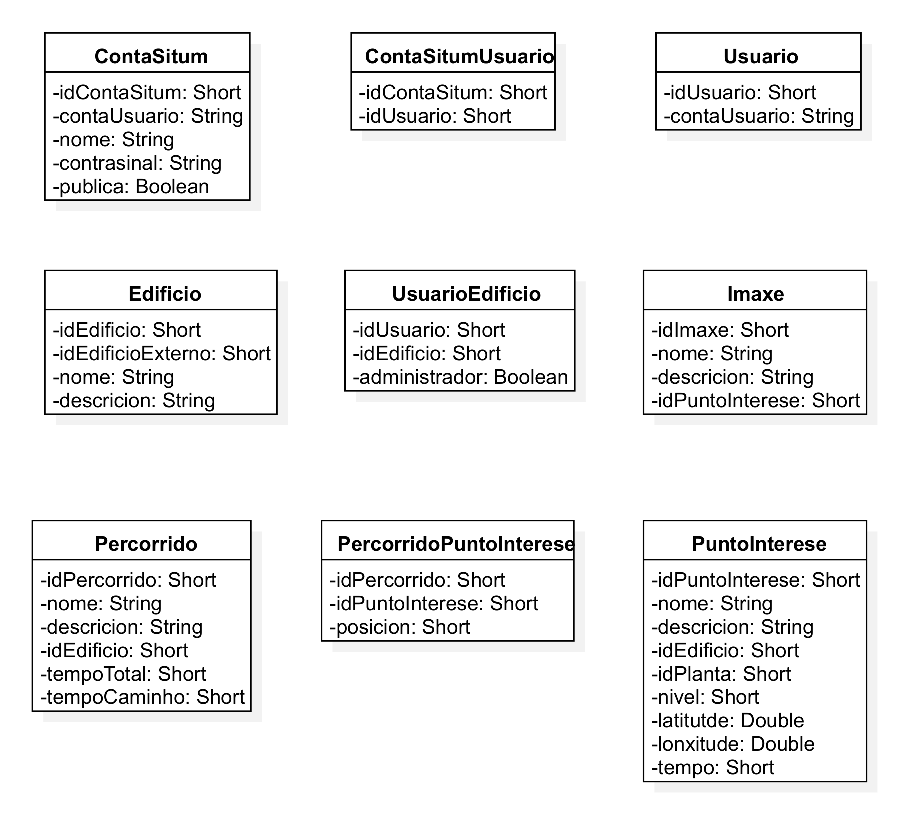
\includegraphics[width=0.95\textwidth]{figures/BD/diagramaEntidades}
		\caption{Diagrama de clases coas entidades.}
		\label{fig:entidades}
	\end{center}
\end{figure}

\begin{figure}[tb] 
	\begin{center}
		\includegraphics[width=0.95\textwidth]{figures/BD/diagramaDaos}
		\caption{Diagrama de clases cos DAOs.}
		\label{fig:daos}
	\end{center}
\end{figure}


\subsection{Transaccionalidade}
Ningunha aplicación está libre de que se produza algún erro na súa execución, ben sexa por culpa de erros na implementación ou por elementos externos (caídas de conexións, erros na base de datos, etc...), polo que é preciso ter en conta estas situacións á hora de realizar modificacións sobre a base de datos para evitar a existencia de información errónea. Cando se realizan modificacións en serie sobre a base de datos que requiren da intervención de varias táboas pode ocorrer un erro xusto no medio, provocando que algunhas táboas fosen modificadas e outras non. Neste caso romperíase a integridade dos datos. Para evitar isto, búscase un sistema que permita que se realicen esas modificacións como se fosen unha soa, e no caso de que se produza un erro, que se desfagan os cambios.
Impleméntase esta transaccionalidade na capa Manager. Non todos os métodos provocan escrituras en base de datos, polo que non será necesario indicar este tipo de transaccionalidade que provoca desfacer cambios en todos eles. O resto marcaranse como de só lectura para non sobrecargar innecesariamente o sistema.

\todo{exemplo de etiqueta}

\subsection{API REST}
A API utilizada para os servizos web é REST, polo que o formato dos datos enviados e recibidos son, na súa maioría JSON. A única excepción prodúcese no envío de imaxes (multipart?).

Estrutura das chamadas: /sw/museo/resto_da_chamada
						/sw/imaxe/resto_da_chamada

Seguridade básica: hai que enviala en cada chamada porque REST é stateless.


/sw/museo/edificios
Recupera todos os edificios dispoñíbeis na plataforma.
GET


/pois/{idEdificioExterno}
Recupera todos os POIs a partir do identificador dun edificio. O identificador é o de Situm
GET


/contas
Recupera todas as contas de Situm públicas, é dicir, as dispoñíbeis para os usuarios anónimos.
GET


/contas/{idUsuario}
Recupera as contas de Situm dispoñíbeis para un usuario, tanto as públicas como as privadas.
GET


/percorridos/{idEdificio}
Recupera os percorridos dun edificio.
GET


/percorridosidexterno/{idEdificioExterno}
Recupera os percorridos dun edificio a partir do seu identificador de Situm.
GET


/ppi/{idPercorrido}
Recupera os POIs (coas súas posicións) dun percorrido a partir do seu identificador.
GET


/percorrido/gardar
Crea ou modifica un percorrido
POST - PUT?


/comprobarUsuarioGoogle
Comproba a validez da autenticación de Google dun usuario. Se é a primeira vez que se autentica, crea o usuario en BD. Devolve información.
POST - PUT?


/poi/gardar
Crea ou modifica un POI
POST - PUT?


/percorrido/eliminar
Elimina un percorrido
POST


/poi/eliminar
Elimina un POI
POST


/imaxe/recuperar/{listaIdImaxeCSV}
Recupera unha lista de imaxes. A entrada está separada por comas.
GET


/recuperar/{idEdificio}/{idPoi}/{idImaxe}




/subir/{idEdificio}/{idPoi}/{nome}/{descricion}



/actualizar/{idImaxe}/{nome}/{descricion}



/eliminar/{idImaxe}


\subsubsection{JSON}


\section{Aplicación Android}
Unha das primeiras decisións á hora de crear unha aplicación Android débese tomar sobre a utilización ou non de fragmentos. Apostouse por unha aplicación que utilizase varias actividades cunha única excepción, o fragmento onde se mostra o mapa de Google Maps. Esta decisión adoptouse debido á maior complexidade que adquire o código co tratamento de fragmentos e o pouco proveito que se lles sacaría nesta aplicación.

A aplicación non ten un gran número de actividades debido a que case toda a lóxica recae sobre a actividade que contén o mapa. A continuación describimos cada unha das actividades incluídas na aplicación.

A actividade inicial permite a autenticación a través de Google e a selección da conta de Situm utilizada que permitirá o acceso a certos edificios. As contas dispoñíbeis estarán restrinxidas en base á conta coa que se autentique o usuario, polo que non sempre se verán as mesmas. Hai algunhas que son públicas polo que estarán dispoñíbeis para todos os usuarios da aplicación.

A principal actividade é MapaActivity, onde se mostra o mapa e se realizan a maioría das accións. É a actividade na que o usuario pasará máis tempo e onde se require amosar maior información, polo que tamén é a máis complexa. Nesta actidade incluíse o fragmento de Google Maps.

Creáronse unha serie de actividades dirixidas a amosar certa información dos puntos de interese e percorridos dos edificios cunha estrutura semellante: DetallePoiActivity e DetallePercorridoActivity. Nelas obsérvanse os datos propios deses elementos, permitindo a súa modificación e borrado nos xa existentes, e tamén a súa creación no caso de non existir previamente se o usuario ten permisos para realizar esas accións.





Clases propias da aplicación que non teñen unha equivalencia exacta co modelo da base de datos, senón que se rexen pola estrutura recibida no JSON.



Un diagrama coa navegación entre pantallas


\subsection{Comunicación co servidor}

\subsection{Comunicación con Situm}
No paquete servizo están as clases que realizan as chamadas tanto ao noso servidor como aos servidores de Situm (paquete interno chamado situm). Unha clase por cada chamada para non mesturar lóxica distinta.

A comunicación con Situm só se realiza dende a aplicación Android.

Escolleuse unha única aplicación tanto para a consulta como para a edición para aproveitar a potencia que nos dá o mapa de interiores á hora de localizar os puntos desexados e marcalos directamente.


Lista de permisos necesarios para a execución.


\section{Sistema de autenticación (GoogleAuth)}
